\section{Adiabatic quantum computation}
%%%%%%%%%%%%%%%%%%%%%%%%%%%%%%%%%%%%%%%%%%%%%%%%%%%%%%%%%%%%%%%%%%%%%%%%%%%%%%%%
\subsection{Classical Ising model}
%%%%%%%%%%%%%%%%%%%%%%%%%%%%%%%%%%%%%%%%%%%%%%%%%%%%%%%%%%%%%%%%%%%%%%%%%%%%%%%%
\begin{frame}{Classical Ising model}
Let the energy function be given (Hamiltonian):
$$
H(s) = - \sum_{i\in \mathcal{I}} h_i s_i - \sum_{(i,j)\in \mathcal{I}\times \mathcal{I}} J_{ij} s_i s_j,
$$
where
$$
s = [s_i]_{i\in \mathcal{I}} \in \{-1, 1\}^{\mathcal{I}}, h_i\in \mathbb{R}, J_{ij}\in \mathbb{R}.
$$
Our goal is to find
$$
s^\star=\min_{s} H(s).
$$
That is the so-called state minimum energy state.
\end{frame}
%%%%%%%%%%%%%%%%%%%%%%%%%%%%%%%%%%%%%%%%%%%%%%%%%%%%%%%%%%%%%%%%%%%%%%%%%%%%%%%%
\subsection{Ising model applications in the computer science}
\foreach \x in {1,2}{
\begin{frame}{Ising models and NP class problems}
\begin{center}
    \includegraphics[page=\x, width=0.65\textwidth]{pics/ising_np.pdf}
\end{center}
\source{Andrew Lucas, \emph{Ising formulations of many NP problems}, Front. Phys. 2014}
\end{frame}
}
%%%%%%%%%%%%%%%%%%%%%%%%%%%%%%%%%%%%%%%%%%%%%%%%%%%%%%%%%%%%%%%%%%%%%%%%%%%%%%%%
\subsection{Quantum Ising model}
%%%%%%%%%%%%%%%%%%%%%%%%%%%%%%%%%%%%%%%%%%%%%%%%%%%%%%%%%%%%%%%%%%%%%%%%%%%%%%%%
\begin{frame}{Quantum (simplified) Ising model}
\begin{block}{Problem Hamiltonian}
We have a given problem Hamiltonian
$$
H_p = - \sum_{i\in \mathcal{I}} h_i \sigma_z^{(i)} - \sum_{(i,j)\in \mathcal{I}\times \mathcal{I}} J_{ij} \sigma_z^{(i)}  \sigma_z^{(j)},
$$
where
$$
\sigma_{\{x,z\}}^{(i)} = \mathbb{1}_2^{\otimes (i-1)} \otimes \sigma_{\{x,z\}} \otimes \mathbb{1}_2^{\otimes (|\mathcal{I}|-i-1)}
$$
$$
\mathbb{1}_2 = /
\begin{pmatrix}
1 & 0\\
0 & 1
\end{pmatrix},
\sigma_z = 
\begin{pmatrix}
1 & 0\\
0 & -1
\end{pmatrix},
\sigma_x = 
\begin{pmatrix}
0 & 1\\
1 & 0
\end{pmatrix}.
$$
\end{block}
\end{frame}
\subsection{Quantum adiabatic protocol}
\begin{frame}[allowframebreaks]{Quantum adiabatic protocol}
\begin{block}{Initial Hamiltonian}
We have a given initial Hamiltonian
$$
H_0 = - \sum_{i\in \mathcal{I}} h_i \sigma_x^{(i)}.
$$
\end{block}

\begin{block}{Effective variable in time Hamiltonian}
$$
H(t) = (1 - \frac{t}{\tau}) H_0 + \frac{t}{\tau} H_p
$$
\end{block}

\framebreak
\begin{block}{Hamiltonian eigenstates}
Each Hamiltonian has its energies $E_n$ ($E_0 \leq E_1 \leq \ldots \leq E_n$) 
and respective eigenstates $\ket{\psi}_n$:
$$
H\ket{\psi}_n = E_n \ket{\psi}_n.
$$
\end{block}

If we start in the state
$$\ket{\psi^{(0)}}_0: H_0\ket{\psi^{(0)}}_0 = E_0^{(0)} \ket{\psi^{(0)}}_0 =
\left(\frac{1}{\sqrt{2}}(\ket{0}-\ket{1})\right)^{\otimes |\mathcal{I}|},
$$
then for large $\tau$ we will end in a state:
$$\ket{\psi^{(p)}}_0: H_p\ket{\psi^{(p)}}_0 = E_0^{(p)} \ket{\psi^{(p)}}_0.$$

\framebreak
In the end, we measure
$$\left\{P_{\pm 1}^{\otimes|\mathcal{I}|}\right\},$$ gdzie
$$\{P_{-1} = \ketbra{0}{0}, P_{1} = \ketbra{1}{1}\}.$$
As a result of the measurement, we get a string
$$s = \{\pm 1\}^{|\times{I}|},$$
which is a solution to our optimization problem.
\end{frame}
%%%%%%%%%%%%%%%%%%%%%%%%%%%%%%%%%%%%%%%%%%%%%%%%%%%%%%%%%%%%%%%%%%%%%%%%%%%%%%%%
\begin{frame}[allowframebreaks]{Adiabatic evolution example}
\begin{center}
    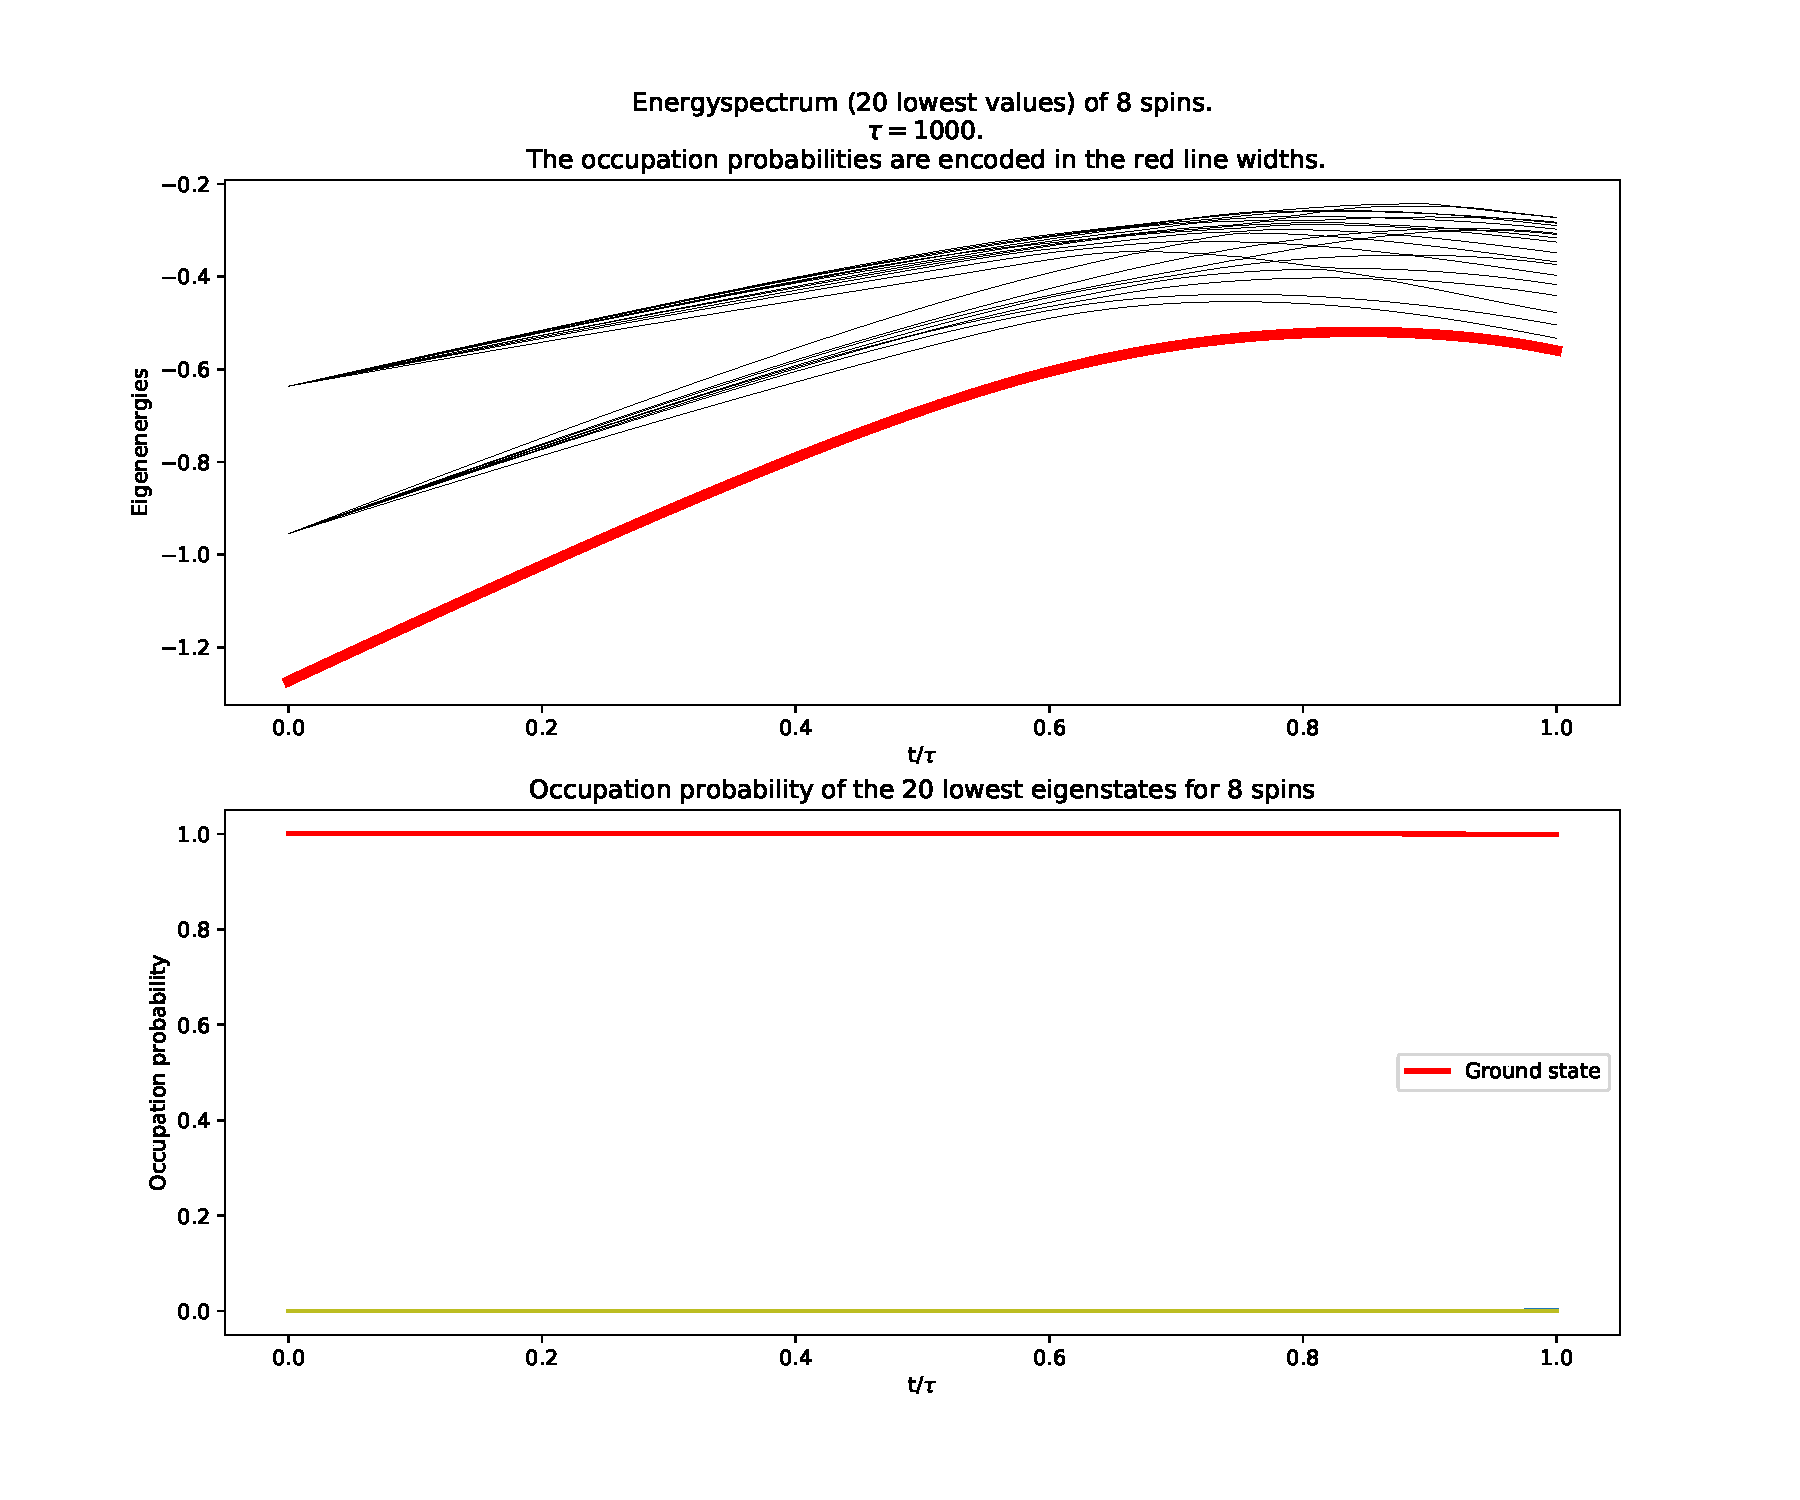
\includegraphics[height=0.75\textheight]{pics/adiabatic/adiabatic_1000.pdf}\\
    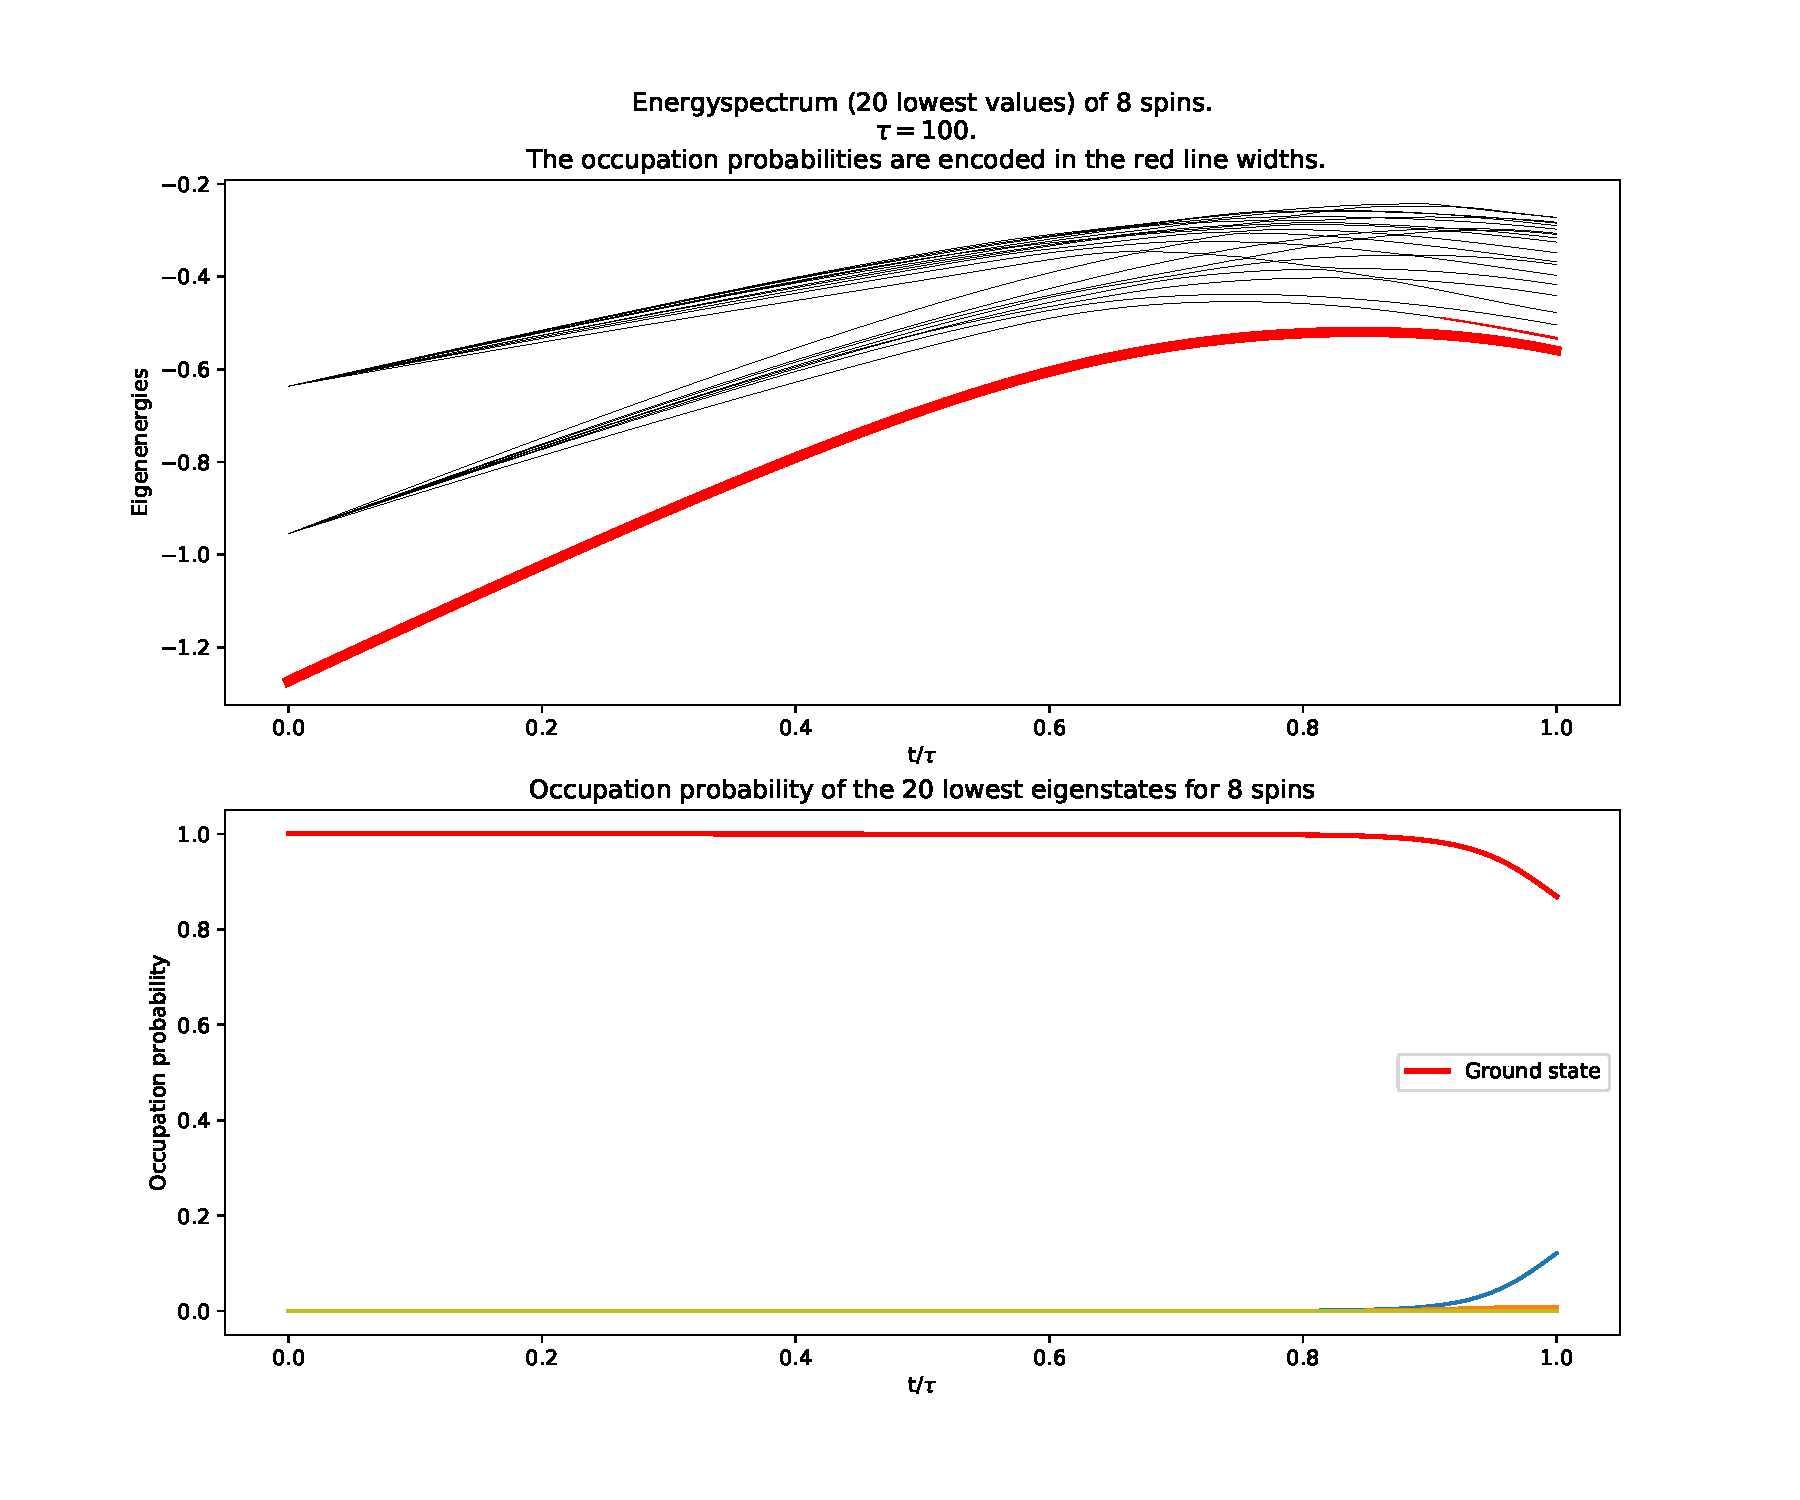
\includegraphics[height=0.75\textheight]{pics/adiabatic/adiabatic_100.pdf}\\
    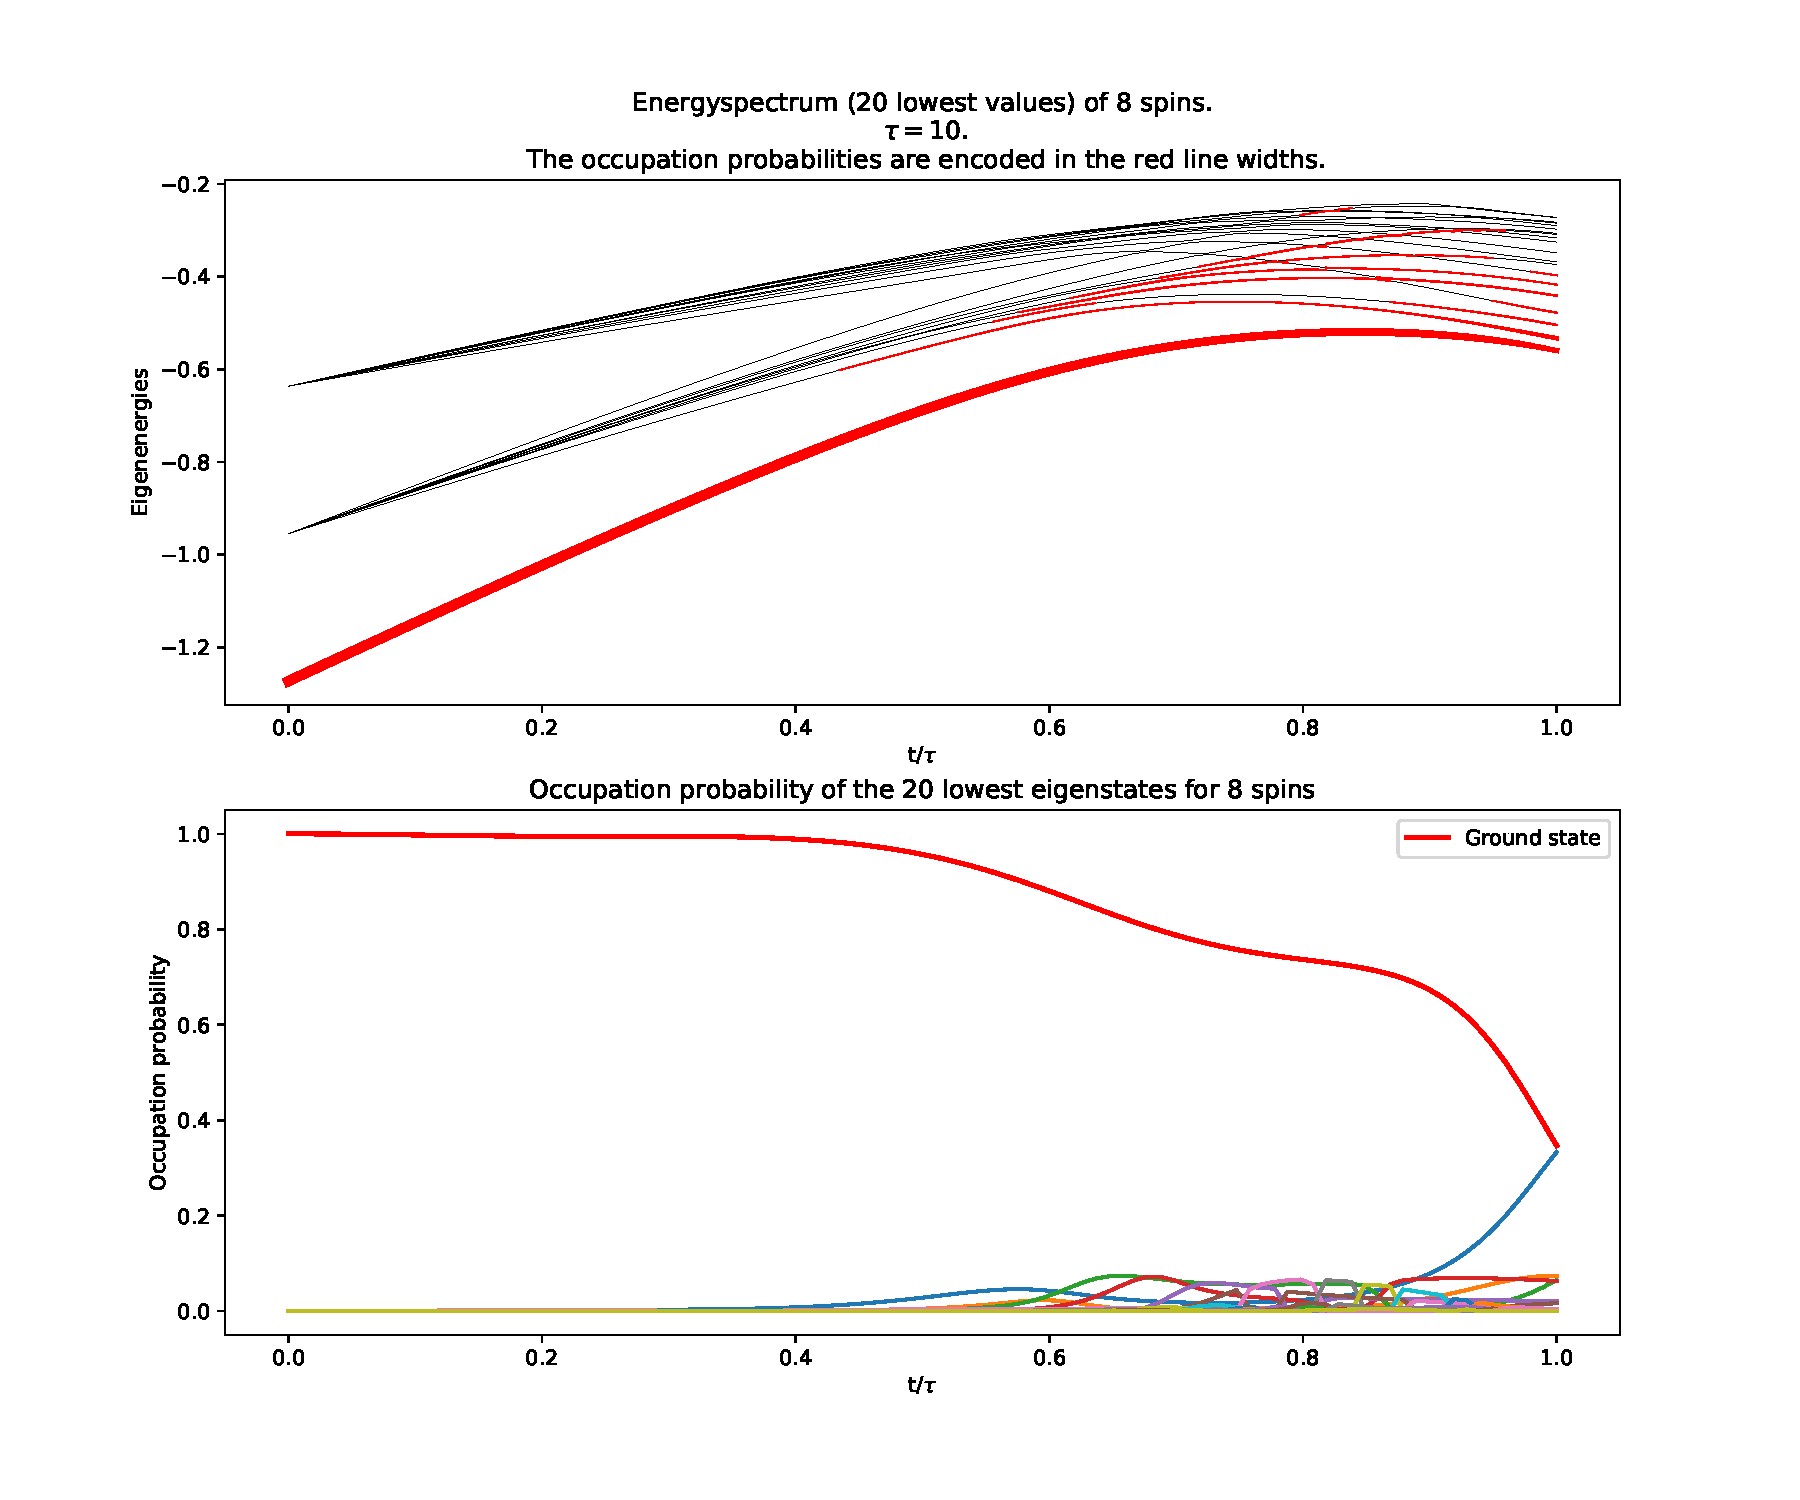
\includegraphics[height=0.75\textheight]{pics/adiabatic/adiabatic_10.pdf}\\
    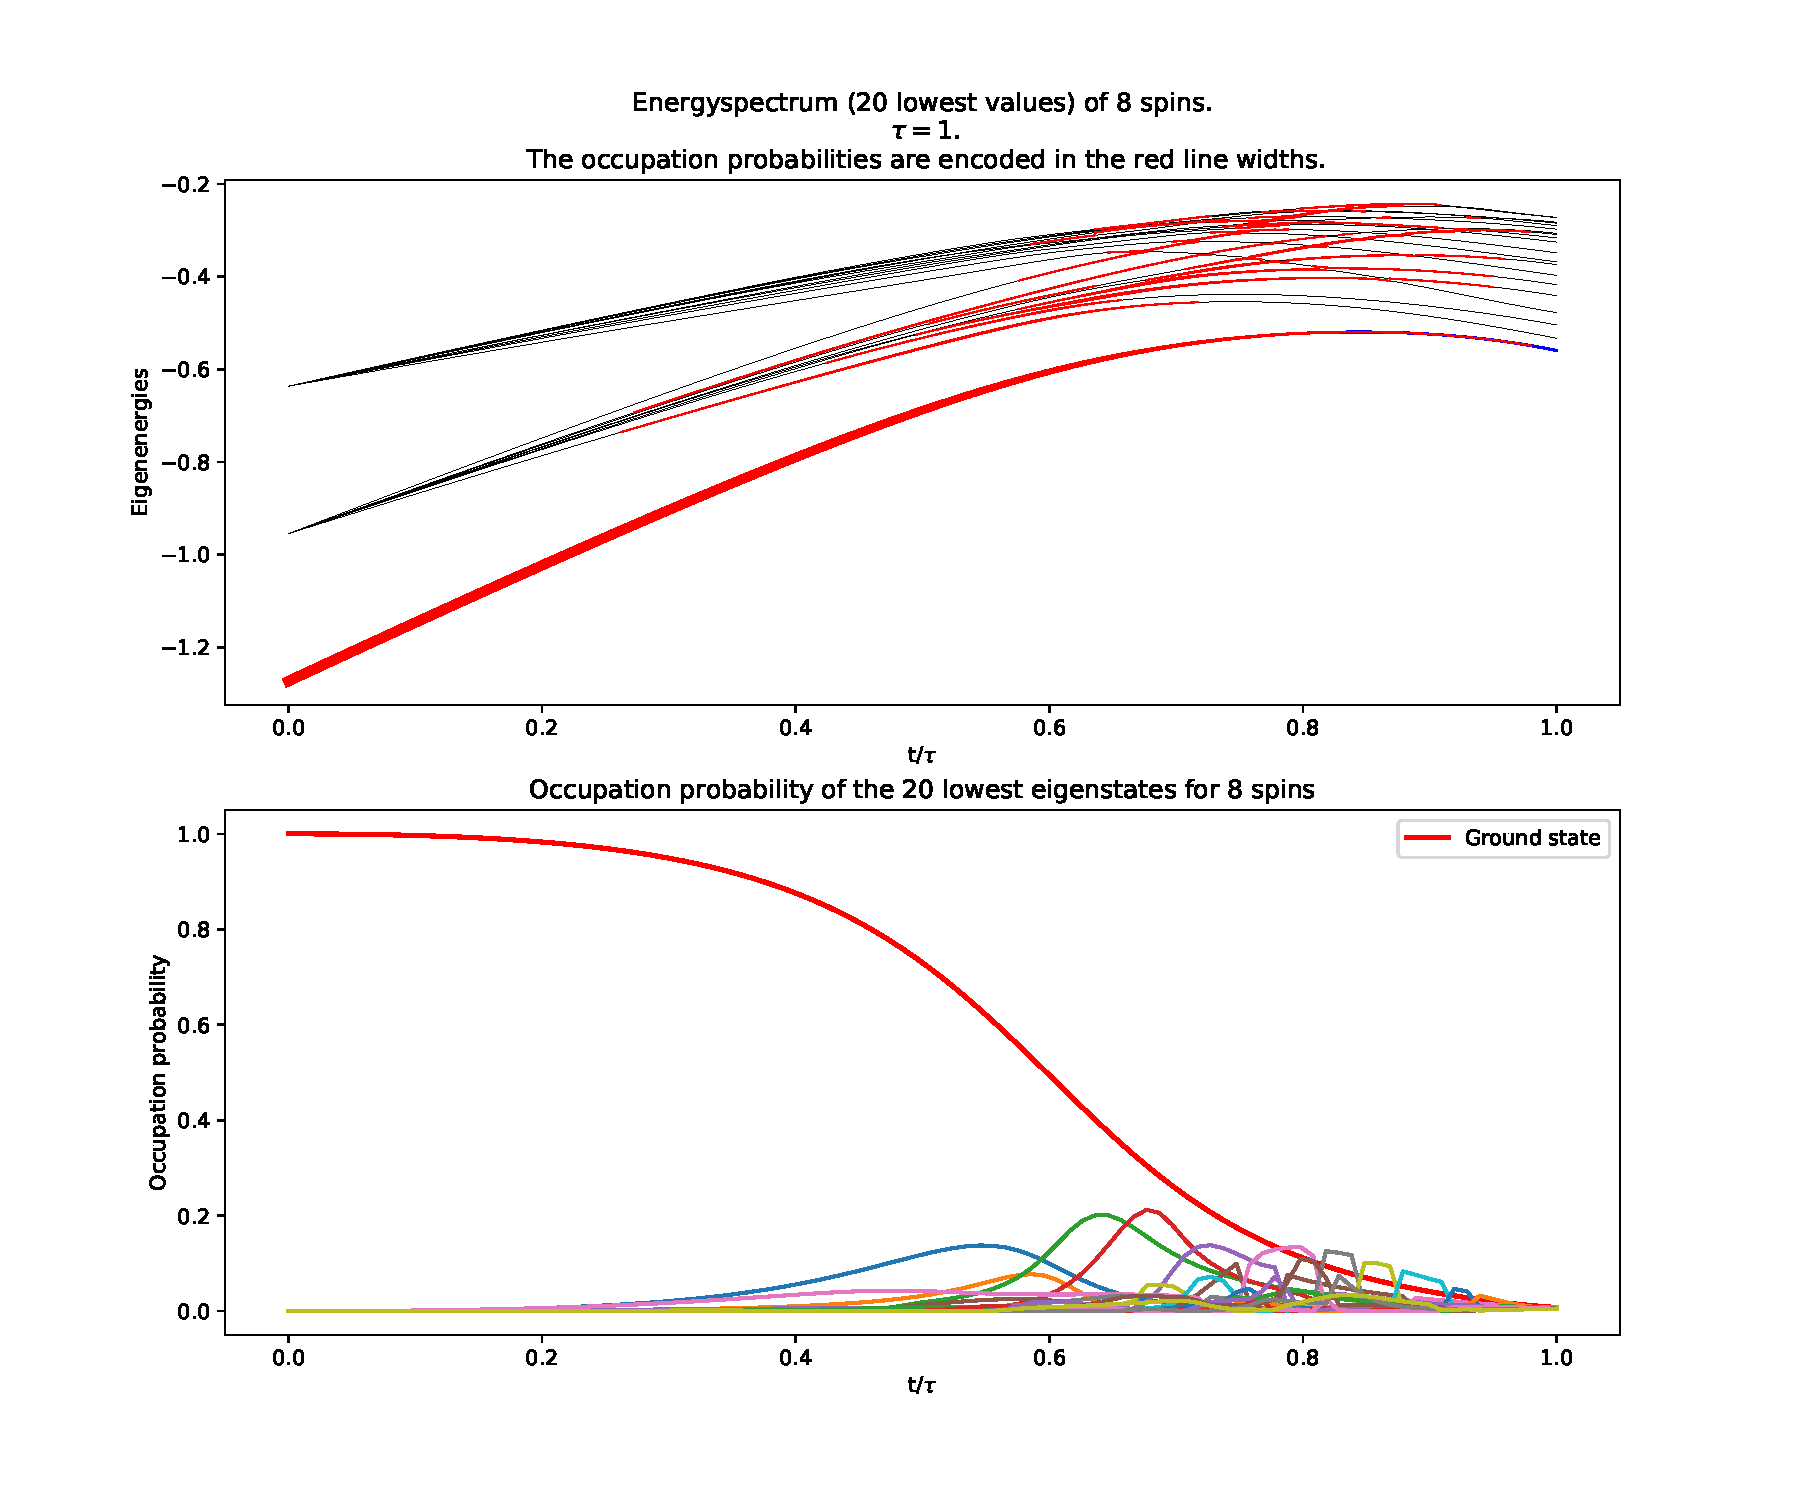
\includegraphics[height=0.75\textheight]{pics/adiabatic/adiabatic_1.pdf}
\end{center}
\end{frame}
%%%%%%%%%%%%%%%%%%%%%%%%%%%%%%%%%%%%%%%%%%%%%%%%%%%%%%%%%%%%%%%%%%%%%%%%%%%%%%%%
\begingroup
\nologo
\begin{frame}{D-Wave annealer 2000Q --- Chimera architecture}
    \begin{center}
    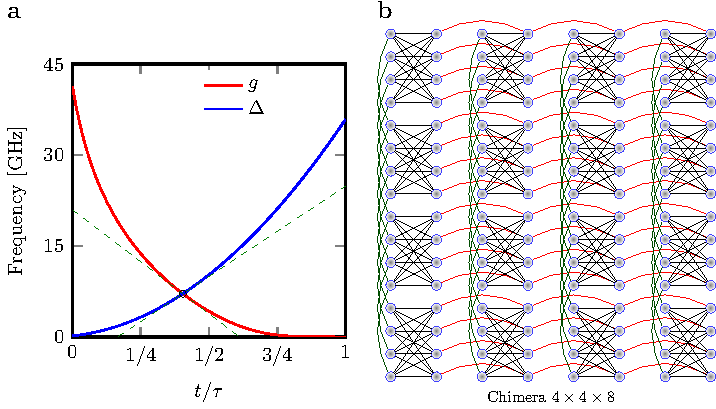
\includegraphics[width=0.5\textwidth]{pics/adiabatic/Fig_1.pdf}\\
    $H(t)/(2\pi\hbar)= -g(t) \sum_{i} \sigma^{(i)}_x -\Delta(t) H_p,
                \quad
                t \in [0, \tau].$
    \end{center}

    \source{B. Gardas}
\end{frame}
\endgroup
%%%%%%%%%%%%%%%%%%%%%%%%%%%%%%%%%%%%%%%%%%%%%%%%%%%%%%%%%%%%%%%%%%%%%%%%%%%%%%%%
\section{Application of D-Wave annealer for spectral image classification post-processing}
%%%%%%%%%%%%%%%%%%%%%%%%%%%%%%%%%%%%%%%%%%%%%%%%%%%%%%%%%%%%%%%%%%%%%%%%%%%%%%%%
\subsection{Chimera architecture}
%%%%%%%%%%%%%%%%%%%%%%%%%%%%%%%%%%%%%%%%%%%%%%%%%%%%%%%%%%%%%%%%%%%%%%%%%%%%%%%%
\begin{frame}{Dwave-2000Q architecture}
    \centering
    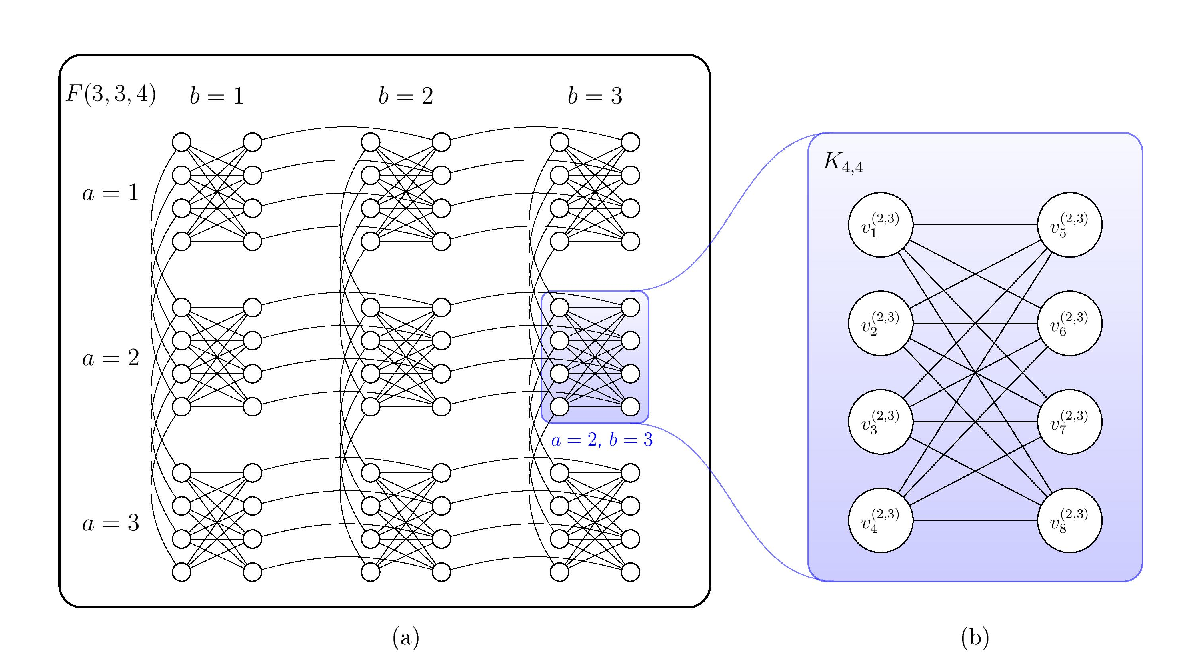
\includegraphics[width=0.8\textwidth]{pics/adiabatic/chimera.pdf}
    \source{arXiv:1608.08547}
\end{frame}
%%%%%%%%%%%%%%%%%%%%%%%%%%%%%%%%%%%%%%%%%%%%%%%%%%%%%%%%%%%%%%%%%%%%%%%%%%%%%%%
\subsection{D-Wave Zephyr architecture}
%%%%%%%%%%%%%%%%%%%%%%%%%%%%%%%%%%%%%%%%%%%%%%%%%%%%%%%%%%%%%%%%%%%%%%%%%%%%%%%
\begin{frame}{New D-Wave topology --- Zephyr \footcite{Boothby2021}}
    \begin{center}
        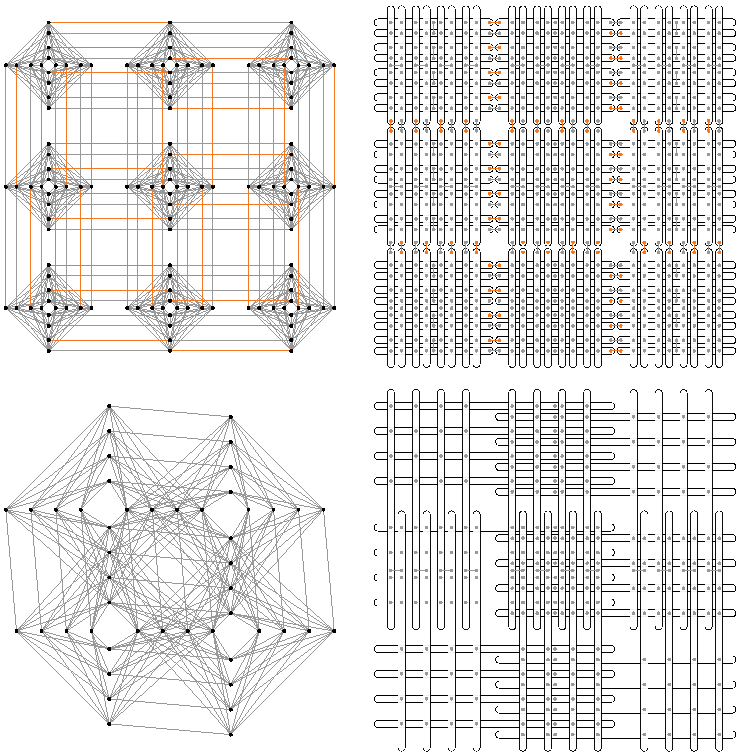
\includegraphics[width=0.43\textwidth, page=1]{pics/adiabatic/zephyr.pdf}
        \includegraphics[width=0.43\textwidth, page=2]{pics/adiabatic/zephyr.pdf}
    \end{center}
\end{frame}
%%%%%%%%%%%%%%%%%%%%%%%%%%%%%%%%%%%%%%%%%%%%%%%%%%%%%%%%%%%%%%%%%%%%%%%%%%%%%%%
\subsection{Problems with Ising solvers}
%%%%%%%%%%%%%%%%%%%%%%%%%%%%%%%%%%%%%%%%%%%%%%%%%%%%%%%%%%%%%%%%%%%%%%%%%%%%%%%
\begin{frame}{QUBO/Ising optimization arms race}
    \begin{block}{Challanges}
        \begin{itemize}
            \item There is no proof that D-Wave machines are better than classical computers.
            \item New classical and quantum algorithms and devices are being proposed.
            \item Quantum Adiabatic Optimization Algorithm on gate model-based devices.
            \item Can we deal with noise in quantum annealers?
        \end{itemize}            
    \end{block}
\end{frame}